\providecommand{\main}{..}

\documentclass[../principal]{subfiles}

\begin{document}
\espacio

  Este capítulo muestra los conceptos básicos y necesarios acerca de los sensores biométricos, fundamentos de seguridad, estándares de biometría, hardware embebido y el protocolo MQTT. También se muestra lo más sobresaliente de la historia de la identificación de personas y las características y propiedades de las huellas dactilares.

  \section{Estado del arte}

  La biometría (del griego \emph{bios} vida y \emph{metron} medida) es el estudio  para el reconocimiento único de humanos basados en uno o más rasgos conductuales o rasgos físicos intrínsecos.\cite{libro:tecnologias_biometricas_aplicadas_seguridad}

  La identificación y autenticación de personas por medio de la verificación de los rasgos físicos es una aplicación muy desarrollada dentro del ámbito de las tecnologías de la información. La biometría de identificación por medio de la comparación de huellas dactilares data desde hace alrededor de 100 años y se encuentra entre los medios más usados de identificación de personas en la actualidad, esto se debe al relativo bajo coste de los dispositivos necesarios para capturar la imagen de las huellas dactilares.

  Cada persona tiene rasgos únicos que la diferencian de las demás. Entre estos rasgos podemos encontrar la voz, la forma del rostro, el iris de los ojos, termograma del rostro, mapa de venas de la mano, patrones de la retina y las huellas dactilares.

  Durante la última década se ha observado el avance en la miniaturización y el uso de escáneres de huellas dactilares en dispositivos de uso diario como teléfonos móviles y computadoras portátiles.

  La biometría electrónica, se acaba de incorporar a las transacciones bancarias por medio de identificación de personas en cajeros automáticos, por tanto se puede usar como referencia para aspectos de seguridad dado su alto grado de fiabilidad.

  \subsection{Técnicas de reconocimiento de identidad}

  \subsubsection{Reconocimiento mediante el iris}

  Estas técnicas son tan fiables que se pueden encontrar sensores de iris en aeropuertos internacionales como los de E.E.U.U., Canadá y los demás que forman parte del programa NEXUS y CANPASS Air\footnote{Canadian Passenger Accelerated Service System}.

  Existen varias técnicas que se usan actualmente, entre las cuales se pueden mencionar: las de reconocimiento de cambios espaciales en la estructura de una imagen que destaca los patrones representativos, captura de imágenes basadas en la reflexión especular de la córnea, filtros artificiales de color que proveen el discriminante ortogonal para el discriminante espacial de patrones.\cite{web:reconocimiento_iris}

  \subsubsection{Forma de las manos}

  Algunas de las técnicas utilizadas para reconocer la forma de las manos son por ejemplo: realizar transformaciones euclidianas para separar y reconocer dedos rígidos para introducir un modelo elíptico que representa los dedos y busca la alineación de los mismos, descomposición de imágenes en sub-bandas de frecuencias para su procesamiento.\cite{tesis:verificacion_identidad_universidad_peru}

  \subsubsection{Contorno del rostro}

  Las técnicas que se utilizan para detectar rostros se basan en el análisis y combinación de imágenes de luz visible e imágenes de luz infrarroja, de las cuales se puede realizar el procesamiento mediante técnicas de reconocimiento 2D y 3D, con los métodos holísticos donde cada pixel es una característica, métodos geométricos que comparan vectores característicos extraídos del perfil y métodos tridimensionales que comparan características mediante múltiples imágenes tomadas con un sistema multi-cámara.\cite{web:reconocimiento_facial}

  \subsubsection{Huellas dactilares}

  Se obtienen todos los rasgos únicos de las huellas, para luego hacer un balance entre la maximización del número de correspondencias y minimización total de los rasgos entre todas las huellas almacenadas de referencia.\cite{tesis:verificacion_identidad_universidad_peru}

  \section{Sensores biométricos de huella dactilar}

  Los sensores biométricos de huellas dactilares o sensores digitales son dispositivos sensibles al tacto que pueden leer, guardar e identificar un número limitado de huellas dactilares.

  \subsection{Clasificación de sensores}

  \begin{description}[align=left]
    \item[Ópticos reflexivos:] Constan de un prisma iluminado por un LED\footnote{Light-Emitting Diode}. Cuando las crestas de las huellas del dedo tocan la superficie, la luz es absorbida, mientras que entre dichas crestas se produce una reflexión total. La luz resultante y las zonas de oscuridad son registradas en un sensor de imagen.\cite{web:sensor_huella_digital}
    \item[Ópticos transmisivos:] Esta técnica funciona sin contacto directo entre el dedo y la superficie del sensor. La luz pasa a través del dedo desde la cara de la uña y al otro lado una cámara toma una imagen directa de la huella dactilar. El sensor vé a través de la superficie de la piel sobre una superficie más profunda y produce una imagen multi-espectral. El uso de diferentes longitudes de onda para generar imágenes nos proporciona información de diferentes estructuras subcutáneas, indicación de que el objeto en cuestión es un dedo genuino.\cite{web:sensor_huella_digital}
    \item[Capacitivos:] El sensor es un circuito integrado de silicio cuya superficie está cubierta por un gran número de elementos transductores (o pixeles), con una resolución típica de 500 dpi. Cada elemento contiene dos electrodos metálicos adyacentes. La capacidad entre los electrodos, que forma un camino de re-alimentación para un amplificador inversor, se reduce cuando el dedo se aplica sobre dicha superficie, se reduce más cuando detecta crestas y menos cuando detecta el espacio entre ellas.\cite{web:sensor_huella_digital}
    \item[Mecánicos:] Se trata de decenas de miles de diminutos transductores de presión que se montan sobre la superficie del sensor. Un diseño alternativo utiliza conmutadores que están cerrados cuando son presionados por una cresta, pero permanecen abiertos cuando están bajo un valle. Esto sólo proporciona un bit de información por pixel, en lugar de trabajar con una escala de grises.\cite{web:sensor_huella_digital}
    \item[Térmicos:] En este caso se detecta el calor conducido por el dedo, el cual es mayor cuando hay una cresta que cuando hay un valle. Se ha desarrollado un componente de silicio con una matriz de pixeles denominado ``FingerChip'', cada uno de los cuales está cubierto con una capa de material piro-eléctrico en el que un cambio de temperatura se traduce en un cambio en la distribución de carga de su superficie. La imagen está en la escala de grises que tiene la calidad adecuada incluso con el dedo desgastado, con suciedad, con grasa o con humedad.\cite{web:sensor_huella_digital}
    \item[De salida dinámica:] El dedo se desplaza lentamente a lo largo del mismo. El sensor sólo dispone de una estrecha zona sensible, y genera una secuencia completa de imágenes, las cuales pueden ser re-ensambladas, mediante un procesador, en una imagen completa. Las prestaciones se mejoran de modo apreciable y se garantiza la eliminación de cualquier grasa residual.\cite{web:sensor_digital}
  \end{description}

  \subsection{Estándares técnicos}

  \begin{description}[align=left]
    \item[CJIS-RS-0010:] Estándar creado en los Estados Unidos por el FBI\footnote{\href{https://www.fbi.gov/}{Federal Bureau of Investigation}}, que define las características técnicas que deben cumplir los escáneres de captura de huellas dactilares (escáneres de papel y los de captura en vivo) y las impresoras de huellas dactilares para asegurar que las imágenes obtenidas cumplan con criterios de calidad mínimos para ser usadas en procesos forenses manuales o automatizados de verificación o identificación dactilar. Actualmente, esta norma se encuentra en su versión 7, actualizada en 1999.\cite{web:huella_dactilar}
    \item[IAFIS-IC-0110:] Estándar creado por el FBI que define el formato para la compresión de imágenes de huellas dactilares conocido como WSQ\footnote{Wavelet Scalar Quantization}. Permite alcanzar niveles de compresión típicos de 15:1, manteniendo los detalles relevantes de la huella dactilar como las minucias y poros. Actualmente, esta norma se encuentra en la versión 3, actualizada en 1997.\cite{articulo:identificacion_forense_comunidades_bacterias}
  \end{description}

  \section{Fundamentos de seguridad}

  El termino seguridad proviene del latín \textsl{securitas} y se usa para definir el concepto de algo donde no se registran peligros, daños ni riesgos. El término seguro define algo firme, cierto e indubitable.\cite{web:seguridad}

  La seguridad, por lo tanto, puede considerarse como una certeza. Desde la prehistoria el hombre ha tratado de buscar seguridad en diferentes ámbitos de su diario vivir, desde tratar de encontrar un refugio donde se sienta a salvo de las inclemencias de la naturaleza, pasando por los candados con los que se impide el acceso a los diferentes ambientes, hasta las bóvedas que resguardan objetos e información confidencial.

  En particular la seguridad informática permite que los recursos del sistema se utilicen de la manera en la que se espera y que quienes puedan acceder a la información sean las personas autorizadas para hacerlo.\cite{web:definicion_seguridad}

  Existen dos tipos de instancias a proteger:
  \begin{itemize}
    \setlength\itemsep{0.1em}
	  \item Los objetos tangibles que se quieren proteger por su valor económico.
	  \item Los objetos intangibles que se quieren proteger por la delicadez de los datos.
  \end{itemize}

  Entonces al trabajar con la seguridad de un recinto, se espera limitar el acceso solo a un cierto número de personas.

  \section{Biometría}

  \begin{wrapfigure}[10]{R}[0pt]{0.4\textwidth}
    \centering
	  \caption{Biometría}
	  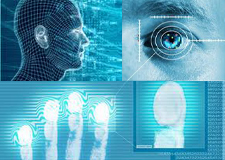
\includegraphics[width=0.3\textwidth]{marco_teorico/biometria.jpg}
	  \caption*{\textbf{Fuente:} \href{http://www.dagospia.com/mediagallery/Dago_fotogallery-154538/761377.htm}{Se avecina el fin del password, Noticias La Repubblica, Italia, 7 de Febrero de 2016}}
  \end{wrapfigure}

  La biometría (del griego \emph{bios} vida y \emph{metron} medida) es el estudio del reconocimiento único de humanos basado en uno o más rasgos conductuales o rasgos físicos intrínsecos.\cite{libro:tecnologias_biometricas_aplicadas_seguridad}

  En un sistema de Biometría típico, la persona se registra con el sistema cuando una o más de sus características físicas y/o de conducta es obtenida, procesada por un algoritmo numérico, e introducida en una base de datos. Idealmente, cuando es identificada, casi todas sus características concuerdan; entonces cuando alguna otra persona intenta identificarse, no empareja completamente, por lo que el sistema no la identifica. Las tecnologías actuales tienen tasas de acierto que varían desde valores bajos como el 60\%, hasta altos como el 99,9\%.
  
  El rendimiento de una medida biométrica se define generalmente en términos de tasa de falso positivo (False Acceptance Rate o FAR), la tasa de falso negativo (False NonMatch Rate o FNMR, también False Rejection Rate o FRR), y la tasa de fallo de alistamiento (Failure-to-enroll Rate, FTE o FER).

  \section{Huella dactilar}

  Se denomina dactilograma o lofograma papilar al conjunto de características provenientes de los dedos de la mano. Los dactilogramas se pueden clasificar de tres formas:

  \begin{itemize}
    \setlength\itemsep{0.1em}
	  \item Dactilograma natural: es el que está en la yema del dedo, formado por las crestas papilares de forma natural.
	  \item Dactilograma artificial: es el dibujo que aparece como resultado al entintar un dactilograma natural e imprimirlo en una zona idónea.
    \begin{figure}[H]
      \centering
      \caption{SmartID, autenticación segura}
      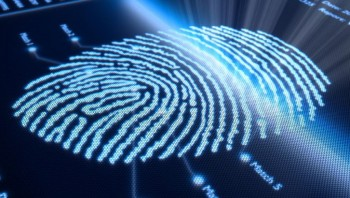
\includegraphics[width=0.3\textwidth]{marco_teorico/huella.jpg}
      \caption*{\textbf{Fuente:} \href{http://www.digitalsecuritymagazine.com/2015/02/24/telefonica-apuesta-por-un-ecosistema-digital-seguro-basado-en-la-biometria/}{Telefónica apuesta por un ecosistema digital seguro basado en la biometría, Revista Virtual Digital Security Magazine, España, 24 de Febrero de 2015}}
    \end{figure}
	  \item Dactilograma latente: es la huella dejada por cualquier dactilograma natural al tocar un objeto o superficie. Este dactilograma queda marcado, pero es invisible. Para su revelación se requiere la aplicación de un reactivo adecuado.\cite{articulo:identificacion_forense_comunidades_bacterias}
  \end{itemize}

  \subsection{Propiedades físicas de las huellas dactilares}

  Está demostrado científicamente que los dibujos que aparecen visibles en la epidermis son:

  \begin{itemize}
    \setlength\itemsep{0.1em}
    \item Perennes porque, desde que se forman en el sexto mes de la vida intrauterina, permanecen indefectiblemente invariables en número, situación, forma y dirección hasta que la putrefacción del cadáver destruye la piel.
    \item Inmutables, ya que las crestas papilares no pueden modificarse fisiológicamente; si hay un traumatismo poco profundo, se regeneran, y si es profundo, las crestas no reaparecen con forma distinta a la que tenían, sino que la parte afectada por el traumatismo resulta invadida por un dibujo cicatrizal.
    \item Diversiformes, pues no se ha hallado todavía dos impresiones idénticas producidas por dedos diferentes.
    \item Originales, ya que todo contacto directo de los lofogramas naturales producen impresiones originales con características microscópicas identificables del tejido epidérmico. Se puede establecer si fueron plasmadas de manera directa por la persona o si se trata de un lofograma artificial.
  \end{itemize}

  Las crestas papilares son glándulas de secreción de sudor, situadas en la dermis, llamadas glándulas sudoríparas. Constan de un tubo situado en el tejido celular subcutáneo, formado por un glomérulo glandular con un canal rectilíneo, que atraviesa la dermis, y termina en la capa córnea de la epidermis, concretamente en el poro, que es un orificio situado en los lomos de las crestas papilares.

  Una vez que el sudor sale, se derrama por todas las crestas y se mezcla con la grasa natural de la piel; lo que da lugar a que, cuando se toque o manipule un objeto apto para la retención de huellas, las crestas dejen una impresión en el objeto.

  \begin{wrapfigure}[13]{l}[0pt]{0.6\textwidth}
    \centering
%    \vspace{-1em}
    \caption{Anexos cutáneos}
    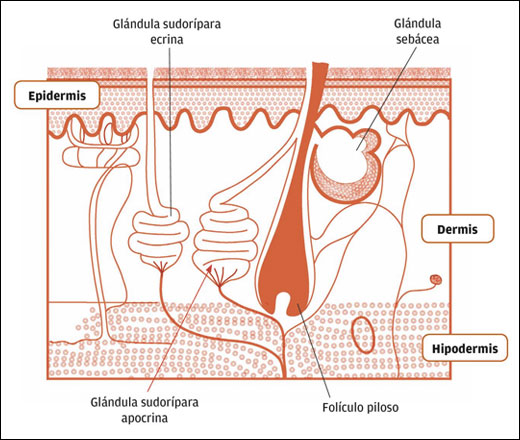
\includegraphics[width=0.55\textwidth]{marco_teorico/glandulas_sudoriparas.jpg}
    \caption*{\textbf{Fuente:} \href{http://www.cosmetologas.com/noticias/val/2247/los-anexos-cutaneos.html}{La Piel de la Web, Revista Virtual Cosmetólogas, Buenos Aires, 14 de Febrero de 2017}}
  \end{wrapfigure}

  Los puntos característicos son las convergencias, desviaciones, empalmes, interrupciones, fragmentos, etcétera, de las crestas y de sus surcos.

  Cuando se cotejan dos huellas dactilares, una dubitada y la otra indubitada; como ejemplo en España, se buscan como mínimo 12 puntos característicos, aunque la obtención de al menos 8 ya tiene validez jurídica.

  Los dibujos o figuras formadas por las crestas papilares reciben el nombre de dactilograma, palabra que deriva de los vocablos griegos; \textsl{daktylos} (dedos) y \textsl{grammas} (escrito). Se denominan dactilogramas papilares si provienen de los dedos de la mano, palmares cuando provienen de la palma de la mano y plantares si provienen de la planta del pie. \cite{articulo:identificacion_forense_comunidades_bacterias}

  \subsection{Características de las huellas dactilares}

  \begin{description}[align=left]
    \item[Cresta:] Son las líneas que sobresalen de la epidermis de forma natural, mismas que forman la impresión de la huella dactilar.
    \item[Valle:] Son los surcos que se forman entre dos crestas, los espacios vacíos o blancos que quedan tras la impresión de la huella.
    \item[Minucia:] Son los puntos característicos que se hallan en la impresión de las huellas, la representación matemática es la siguiente: $ M = \{x, y, \theta\} $, donde (x, y) es un punto o coordenada dentro de la impresión de la huella y $ \theta $ es el ángulo medido en radianes que forma la minucia con el eje $ x $.

    \begin{figure}[H]
      \centering
      \caption{Tipos de minucias}
      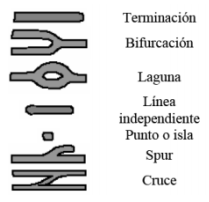
\includegraphics[width=0.25\textwidth]{marco_teorico/tipos_minucias.png}
      \caption*{\textbf{Fuente:} \href{http://ccc.inaoep.mx/~esucar/Clases-mgp/Proyectos/reporte_modelos_huellas.pdf}{Clasificación de huellas digitales mediante minucias, Instituto Nacional de Astrofísica, Óptica y Electrónica, México, Abril de 2009} \cite{reporte:clasificacion_huellas_mediante_minucias}}
    \end{figure}

    \item[Terminación:] Se dá cuando una cresta llega a un punto final y no continua su recorrido.
    \item[Bifurcación:] Se forma cuando una cresta se divide en dos y forma dos crestas que siguen un curso diferente la una de la otra.
    \item[Delta:] Es un lugar específico dentro de la impresión donde dos o tres crestas forman la figura de un triángulo.

    \begin{figure}[H]
      \centering
      \caption{Corazón y Delta}
      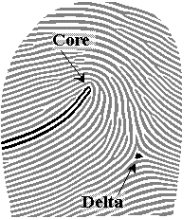
\includegraphics[width=0.2\textwidth]{marco_teorico/corazon_delta.png}
      \caption*{\textbf{Fuente:} \href{http://ccc.inaoep.mx/~esucar/Clases-mgp/Proyectos/reporte_modelos_huellas.pdf}{Clasificación de huellas digitales mediante minucias, Instituto Nacional de Astrofísica, Óptica y Electrónica, México, Abril de 2009} \cite{reporte:clasificacion_huellas_mediante_minucias}}
    \end{figure}

    \item[Corazón:] Es la convergencia donde se pueden hallar muchas terminaciones de crestas
  \end{description}

  \subsection{Tipos de huellas dactilares}

  \begin{description}[align=left]

    \begin{figure}[H]
      \centering
      \caption{Tipos de huellas dactilares}
      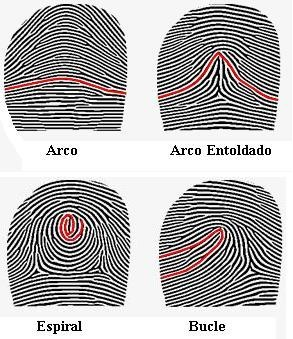
\includegraphics[width=0.3\textwidth]{marco_teorico/tipo_huella_dactilar.jpg}
      \caption*{\textbf{Fuente:} \href{http://dis.um.es/~lopezquesada/documentos/IES_1213/SAD/curso/UT3/ActividadesAlumnos/12/enlaces/biometricos.html}{Patrones de Pukinje, Sistemas Biométricos, Juan Segura Martínez, Revista Virtual Seguridad Pasiva, 2012}}
    \end{figure}

    \item[Bucle:] En este patrón las líneas en el reborde exterior que llegan al centro de la impresión dactilar se curvan y continúan en bucle hasta llegar nuevamente al mismo reborde; por esta razón solo se halla un delta en este tipo de patrones. 65\% de la población mundial tiene este tipo de huellas.
    \item[Espiral:] Este patrón contiene 2 o mas deltas, existe una curva ligera antes de comenzar cada delta. Existen cuatro tipos de espiral, la espiral simple, la espiral bolsillo central, el doble bucle y la espiral accidental. 30\% de la población mundial tiene este tipo de huellas.
    \item[Arco:] Es el patrón mas raro, en este tipo de patrones las líneas de cresta son divergentes y van desde un reborde del dedo al otro sin formar deltas. Existen dos tipos de arco, el arco simple que se asemeja a las olas del mar y el arco entoldado o tienda de campaña donde las líneas se curvan de una manera más extrema hacia el centro de la impresión. 5\% de la población mundial tiene este tipo de huellas.
  \end{description}

  \subsection{Aplicaciones}

  Actualmente los sensores biométricos se utilizan en gran número de aplicaciones, por ejemplo en computadoras portátiles y teléfonos inteligentes gracias a su alto grado de reducción de tamaño y su bajo costo económico.

  También se pueden encontrar sensores digitales en discos duros, memorias USB y lectores de tarjetas. Últimamente se han desarrollado dispositivos que requieren de identificación biométrica para realizar transacciones bancarias.

  Se pueden hallar dispositivos para la autenticación a diferentes cuentas en línea por medio de la huella dactilar.\href{http://www.google.com/patents/US20050097338}{\footnote{Memoria Flash USB protegida por biometría, Patente de Google US 20050097338 A1, Kong Lee}}

  Estos sensores además son ampliamente utilizados para el control de personal en empresas o instituciones y para la identificación de personas para los sistemas de apertura de puertas o de marcado de llegadas y salidas para el control del horario laboral.

  \section{Sistemas de hardware embebido}

  Un sistema embebido es un hardware destinado a realizar algunas funciones dedicadas, generalmente orientadas a la computación en tiempo real. Los sistemas embebidos por lo general contienen un procesador de bajo costo y una memoria limitada para el almacenamiento de variables o partes del o los programas. Como parte central se pueden encontrar microprocesadores, procesadores digitales de señales y/o micro-controladores.

  Los sistemas embebidos se comunican con otras interfaces mediante puertos como ser: UART\footnote{Universal Asynchronous Receiver-Transmitter}, SPI\footnote{Serial Peripheral Interface}, $ I^2 $C\footnote{Inter-Integrated Circuit}, USB\footnote{Universal Serial Bus}, Ethernet, Wi-Fi\footnote{Wireless Fidelity}, GSM\footnote{Global System for Mobile}, GPRS\footnote{General Packet Radio Service}, DSRC\footnote{Dedicated Short Range Communications}, etc.

  Las salidas de los sistemas embebidos pueden ser analógicas o digitales y se usan para controlar motores, activar diodos LED, polarizar transistores, activar relés, etc.

  Las entradas pueden ser también analógicas o digitales procedentes de diferentes tipos de sensores. \cite{libro:embedded_system_design}

  \section{Ethernet}

  Ethernet es un sistema de transmisión de datos en banda base, diseñado por Xerox Corporation, a mediados de la década de 1970.

  El subcomité de ANSI e IEEE 802.3 han definido la norma de transmisión Ethernet 10BASE-T que se basa en la topología de estrella. La ``T'' representa ``UTP'', de unshielded twisted-pair
wire, o cable de par de alambres trenzados. Se desarrolló el sistema 10BASE-T para permitir el uso de cableado telefónico existente, de grado de voz, para conducir señales de Ethernet.\cite{libro:sistemas_de_comunicaciones_electronicas}

  La estructura de la trama IEEE 802.3 es la siguiente:

  \begin{table}[h]
    \scriptsize
    \centering
    \caption{Formato de la trama IEEE 802.3}
    \setlength\extrarowheight{2pt}
\noindent\begin{tabular}{C{0.7cm}|C{1.35cm}|C{1.5cm}|C{1cm}|C{1cm}|C{1cm}|C{1cm}|C{1.8cm}|C{1.5cm}|}
  \cline{2-9}
  & Preámbulo & Delimitador de trama de arranque & Dirección de destino & Dirección de fuente & Longitud & Payload & Secuencia de comprobación de trama & Delimitador de fin de trama \\
  \cline{2-9}
  Bytes: & 7 & 1 & 2-6 & 2-6 & 2 & 46-1500 & 4 & 9.6 $ \mu s $ \\
  \cline{2-9}
\end{tabular}
    \caption*{\textbf{Fuente:} Sistemas de comunicaciones electrónicas, Wayne Tomasi, \cite[p.~657]{libro:sistemas_de_comunicaciones_electronicas}}
  \end{table}

  \begin{description}[align=left]
    \item[Preámbulo:] El preámbulo consiste en siete bytes, para establecer la sincronización de los relojes. El último byte del preámbulo se usa como delimitador de la trama de arranque.
    \item[Delimitador de la trama de arranque:] No es más que una serie de dos unos lógicos agregada al final del preámbulo, cuyo objetivo es marcar el final del preámbulo y el principio de la trama de datos.
    \item[Dirección de destino:] Las direcciones de la fuente y el destino forman el encabezado de la trama. La dirección del destino consiste en seis bytes (48 bits) y es la dirección del o los nodos que se han designado para recibir la trama. La dirección puede ser única, de grupo o global y se determina con las siguientes combinaciones:
    \begin{itemize}
      \item bit 0 = 0. Si el bit 0 es un 0, la dirección se interpreta como única, especial para una sola estación.
      \item bit 0 = 1. Si el bit 0 es un 1, la dirección se interpreta como de grupo. Todas las estaciones que tengan preasignada esta dirección de grupo aceptarán la trama.
      \item bit 0 = 47. Si todos los bits en el campo de destino son unos, quiere decir que la dirección es global, y que se identificó a todos los nodos como receptores de esta trama.
    \end{itemize}
    \item[Dirección de fuente:] Esta dirección consiste en seis bytes (48 bits), y corresponden a la dirección de la estación que manda la trama.
    \item[Campo de longitud:] El campo de longitud de 2 bytes indica la longitud del campo de datos de control de enlace lógico (logical link control, LLC), también llamado Payload, que es de longitud variable y contiene incrustados todos los protocolos de capa superior.
    \item[Payload:] El campo de Payload contiene la información, y puede tener de 46 a 1500 bytes de longitud.
    \item[Campo de secuencia de verificación de trama:] El campo CRC (frame check sequence) contiene 32 bits para detección de errores, y se calcula a partir de los campos de encabezado y de datos.
    \item[Delimitador de fin de trama:] El delimitador de fin de trama es un periodo de 9.6 $ \mu s $ en el que no se transmiten bits. En la codificación Manchester, cuando no hay transiciones de longitud mayor que el tiempo de 1 bit, se indica el final de la trama.
  \end{description}

  \subsection{POE (Power Over Ethernet)}

  POE es un estándar IEEE desde el año 2003; éste sistema se compone de un inyector y un receptor conectados mediante un cable ethernet.
  Existen dos estándares, el primero 802.3af o POE activo, funciona con un inyector que realiza una prueba de carga mediante el consumo de corriente al lado del receptor, para verificar si el receptor es un dispositivo POE o no, en caso de no serlo envía los datos entre +/-2.5V; pero si detecta un dispositivo POE; es decir una carga, realiza una prueba, mediante niveles de voltaje, de cual es la potencia necesaria al lado del receptor para enviar los datos entre +/-2.5V conjuntamente con un voltaje de -48V en uno de los pares trenzados que puede ser el par verde o el azul del cable ethernet de categoría 5, 6 o 7; a su vez se cierra el circuito con una referencia en el otro par que puede ser el par naranja o café respectivamente.

  Estos 48V son separados del voltaje de los datos en el lado del receptor y es con este que se alimenta al circuito que requiere energía, no sin antes realizar una conversión DC/DC adecuada a los requerimientos del circuito objetivo.

  \begin{figure}[h]
    \centering
	  \caption{Power Over Ethernet}
	  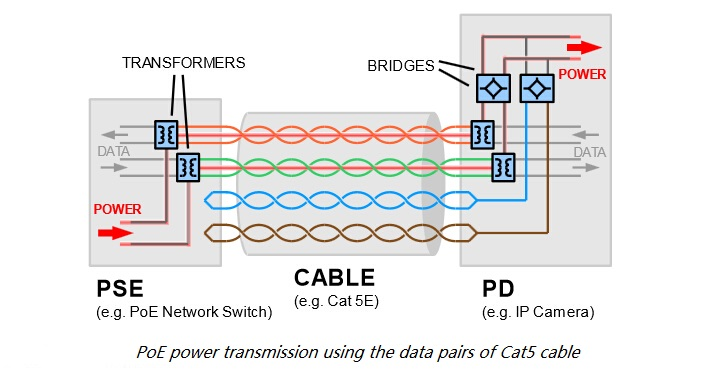
\includegraphics[width=0.95\textwidth]{marco_teorico/poe.jpg}
	  \caption*{\textbf{Fuente:} \href{http://www.fs.com/blog/power-over-ethernet-analysis.html}{Power Over Ethernet Analysis, Blog FS.com, 19 de Enero de 2016}}
  \end{figure}

  El segundo método es el 802.3at o POE pasivo, utiliza cuatro cables para datos y cuatro cables para energía, generalmente se puede encontrar que utiliza el par azul para enviar el voltaje y el par café como referencia, la debilidad de este método es que la velocidad de transmisión/recepción disminuye debido a la eliminación de los dos pares usados para el voltaje, a cambio se puede prescindir del protocolo de reconocimiento de carga del circuito receptor. Cabe mencionar que un inyector 802.3at es compatible con un receptor 802.3af pero no al contrario.

  \section{Software}

  \subsection{Internet de las cosas}

  \begin{figure}[h]
    \centering
	  \caption{Internet de las cosas}
	  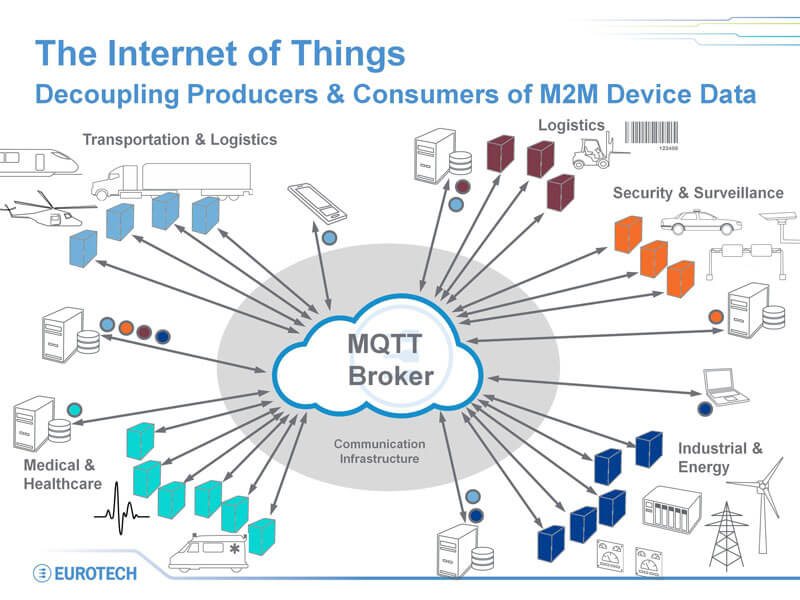
\includegraphics[width=0.85\textwidth]{marco_teorico/conexion_mqtt.jpg}
	  \caption*{\textbf{Fuente:} \href{https://thenewstack.io/mqtt-protocol-iot/}{Get to Know MQTT: The Messaging Protocol for the Internet of Things, Industrias Janakiram \& Associates, 2016}}
  \end{figure}

  El Internet de las Cosas es un concepto que se refiere a la interconexión de dispositivos de la vida cotidiana a una red local o al propio Internet. La mayoría de los dispositivos del Internet de las Cosas capturan información de sensores y envían estos datos a una o más bases de datos, un ejemplo de estos dispositivos son los refrigeradores inteligentes, que verifican la cantidad de alimentos de cada tipo e incluso pueden realizar pedidos de compra directamente a los supermercados cuando un alimento se encuentra por debajo de un límite definido por el usuario. Otro ejemplo son los sensores que se implantan a las vacas en Holanda, éstos recaban la información acerca de la salud, la posición y la edad de las vacas, generando hasta 200MB de datos al año por cada vaca, con estos datos se pueden generar gráficas para mejorar la crianza e incluso predecir y prevenir epidemias de enfermedades bovinas.\cite{reporte:internet_de_las_cosas}

  \begin{figure}[h]
    \centering
	  \caption{Número de dispositivos conectados por persona}
	  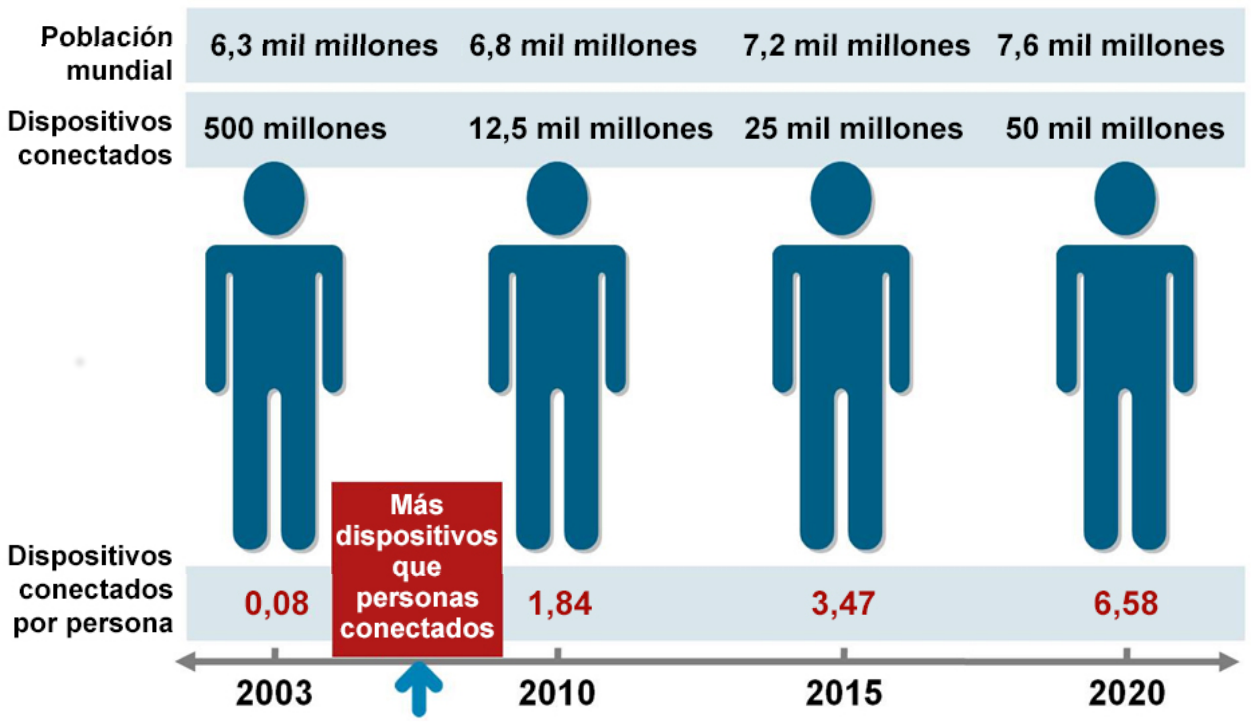
\includegraphics[width=\textwidth]{marco_teorico/dispositivos_conectados.png}
	  \caption*{\textbf{Fuente:} \href{http://www.cisco.com/c/dam/global/es_mx/solutions/executive/assets/pdf/internet-of-things-iot-ibsg.pdf}{Internet de las cosas: Cómo la próxima evolución de Internet lo cambia todo, Dave Evans, Cisco IBSG, 2011}}
  \end{figure}

  Los dispositivos del Internet de las Cosas transmiten los datos mediante una gran gama de protocolos, entre los cuales el más conocido por su eficiencia en cuanto a energía consumida y pequeño tamaño en la trama de paquete de datos es MQTT. Este protocolo es usado en aplicaciones populares como Facebook Messenger, Amazon Web Services, OpenStack y Microsoft Azure entre otras.\cite{web:mqtt}

  \subsection{Entorno de ejecución}

  Un entorno de ejecución es un estado de máquina virtual que suministra servicios para los procesos de un programa de computadora que se está ejecutando. Puede pertenecer al mismo sistema operativo, o ser creado por el software del programa en ejecución.
  
  En la mayoría de los casos, el sistema operativo maneja la carga del programa con una parte del código llamada cargador, haciendo configuración básica de memoria y enlazando el programa con cualquier biblioteca de vínculos dinámicos a la cual haga referencia. En algunos casos un lenguaje o implementación hará esas tareas en lugar del runtime del lenguaje, a pesar de que es inusual en los lenguajes principales sobre los sistemas operativos de usuarios normales.

  Cierta depuración de programas sólo puede realizarse (o ser más eficiente o precisa) cuando se realiza en ejecución. La comprobación de errores lógicos y límites de arrays son algunos ejemplos. Por esta razón, algunos errores de programación no son descubiertos hasta que el programa es probado en un entorno ``en vivo'' con datos reales, a pesar de la comprobación en tiempo de compilación sofisticada y pruebas previas a la publicación. En este caso, el usuario final puede encontrar un mensaje de ``error en tiempo de ejecución'' (runtime error).\cite{web:entorno_ejecucion}

  \subsection{Base de datos}

  Una base de datos es un conjunto de datos pertenecientes a un mismo contexto y almacenados sistemáticamente para su posterior uso. En este sentido; una biblioteca puede considerarse una base de datos compuesta en su mayoría por documentos y textos impresos en papel e indexados para su consulta. Actualmente, y debido al desarrollo tecnológico de campos como la informática y la electrónica, la mayoría de las bases de datos están en formato digital, siendo este un componente electrónico, por tanto se ha desarrollado y se ofrece un amplio rango de soluciones al problema del almacenamiento de datos.

  Las bases de datos pueden ser estáticas, es decir de solo lectura, o dinámicas que cuentan con operaciones de actualización, borrado y edición.

  Las bases de datos relacionales están formadas por ``tuplas'', cada relación genera una tabla que está compuesta por registros (las filas de una tabla), que representan las tuplas, y campos (las columnas de una tabla).

  La información puede ser recuperada o almacenada mediante consultas que ofrecen una amplia flexibilidad y poder para administrar la información. El lenguaje más habitual para construir las consultas a bases de datos relacionales es SQL\footnote{Structured Query Language}.\cite{web:base_de_datos}

  \bibliografia
\end{document}
